%---------------------------------------
\addcontentsline{toc}{chapter}{Galatians}

% Safely inserts your illustration full-bleed on its own page.
% This completely bypasses the page builder, headers, and geometry bugs!
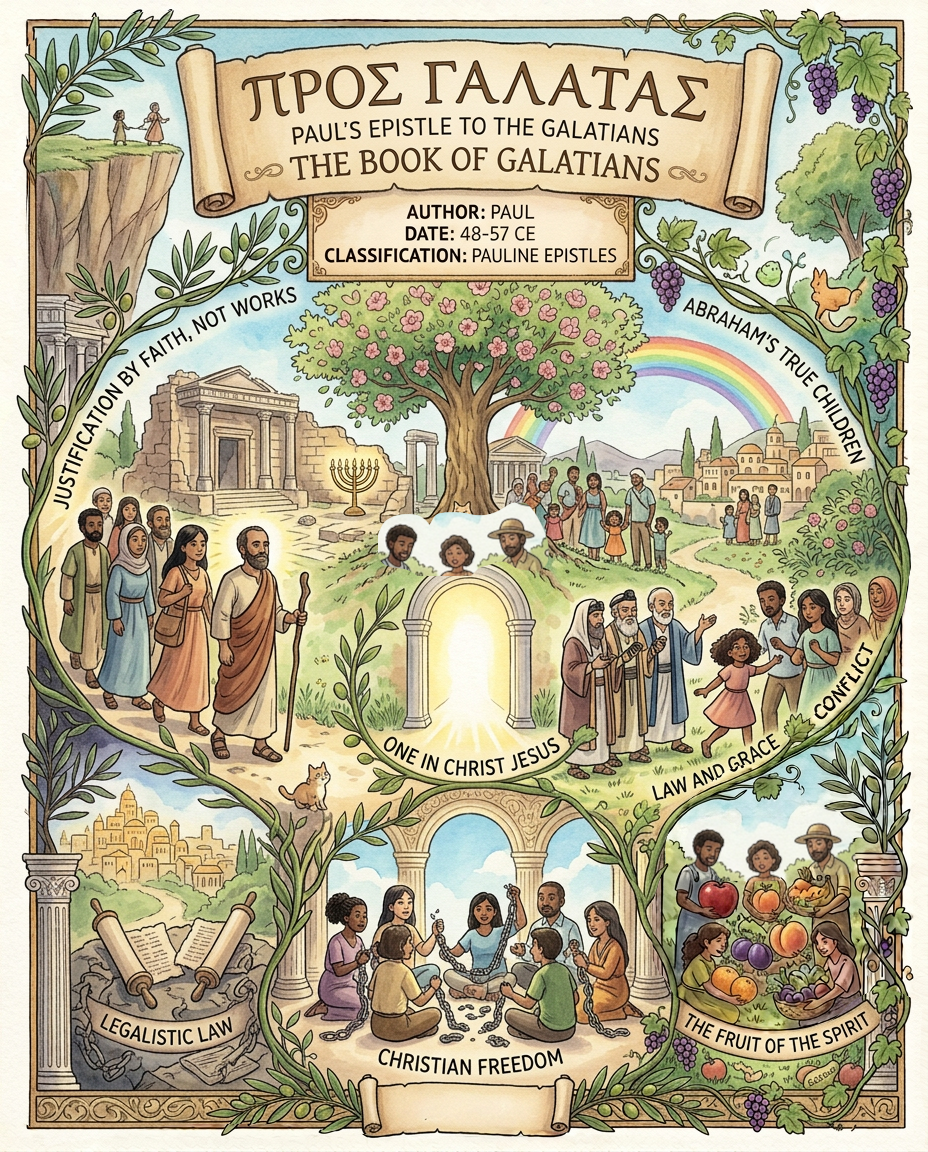
\includepdf[pages=1, fitpaper=false, width=\paperwidth, height=\paperheight, , keepaspectratio=false]{images/divider2/galatians2.png}

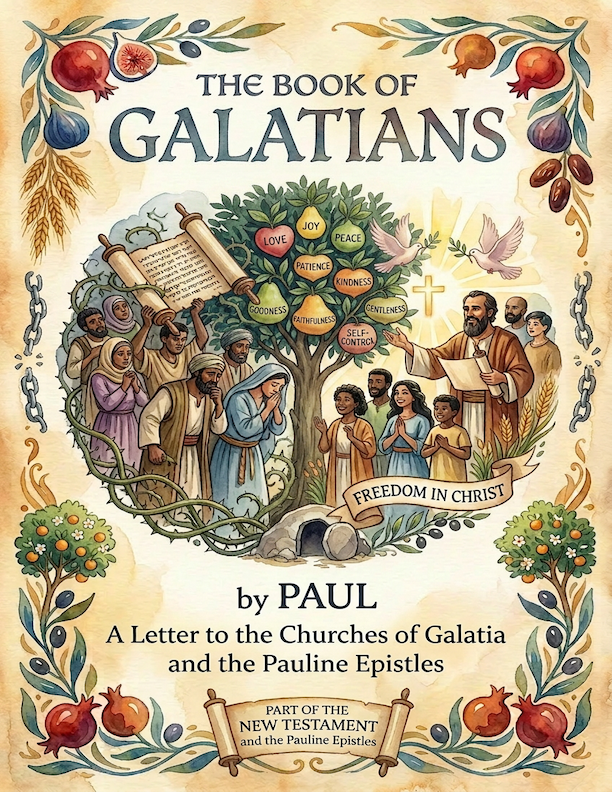
\includepdf[pages=1, fitpaper=false, width=\paperwidth, height=\paperheight, , keepaspectratio=false]{images/divider1/galatians.png}

\includepdf[pages=1, fitpaper=false, width=\paperwidth, height=\paperheight, , keepaspectratio=false]{images/8.5x11-Dot-Grid.png}

\includepdf[pages=1, fitpaper=false, width=\paperwidth, height=\paperheight, , keepaspectratio=false]{images/8.5x11-Dot-Grid.png}

\mybook{Galatians}
\vspace{-1.36in}

\mychapter{} \myverse*{}Paul, an emissary—not from men, nor through man, but through Yeshua the Messiah,\footnote{1:1 “Messiah” means “Anointed One”.} and God the Father, who raised him from the dead—
\myverse{}and all the brothers\footnote{1:2 The word for “brothers” here and where context allows may also be correctly translated “brothers
	and sisters” or “siblings.”
} who are with me, to the assemblies of Galatia:
\myverse{}Grace to you and peace from God the Father and our Lord Yeshua the Messiah,
\myverse{}who gave himself for our sins, that he might deliver us out of this present
evil age, according to the will of our God and Father—
\myverse{}to whom be the glory forever and ever. Amen.

\myverse{}I marvel that you are so quickly deserting him who called you in
the grace of Messiah to a different “good news”,
\myverse{}but there isn’t another “good news.” Only there are some who trouble you and
want to pervert the Good News of Messiah.
\myverse{}But even though we, or an angel from heaven, should proclaim to you any “good
news” other than that which we preached to you, let him be cursed.
\myverse{}As we have said before, so I now say again: if any man preaches to you any “good
news” other than that which you received, let him be cursed.

\myverse{}For am I now seeking the favor of men, or of God? Or am I striving
to please men? For if I were still pleasing men, I wouldn’t be a servant of Messiah.

\myverse{}But I make known to you, brothers, concerning the Good News which
was preached by me, that it is not according to man.
\myverse{}For I didn’t receive it from man, nor was I taught it, but it came to me through
revelation of Yeshua the Messiah.
\myverse{}For you have heard of my way of living in time past in Judaism\footnote{1:13 or, traditional Judaism},
how that beyond measure I persecuted the assembly of God and ravaged it.
\myverse{}I advanced in Judaism\footnote{1:14 or, traditional Judaism} beyond many
of my own age among my countrymen, being more exceedingly zealous for the traditions of my fathers.
\myverse{}But when it was the good pleasure of God, who separated me from my mother’s
womb and called me through his grace,
\myverse{}to reveal his Son in me, that I might proclaim him among the Gentiles, I didn’t
immediately confer with flesh and blood,
\myverse{}nor did I go up to Jerusalem to those who were emissaries before me, but I
went away into Arabia. Then I returned to Damascus.

\myverse{}Then after three years I went up to Jerusalem to visit Peter,
and stayed with him fifteen days.
\myverse{}But of the other emissaries I saw no one except Jacob, the Lord’s brother.
\myverse{}Now about the things which I write to you, behold,\footnote{1:20 “Behold”, from “ἰδοὺ”, means look at, take notice, observe, see, or gaze at. It is often used
	as an interjection.} before God, I’m not lying.
\myverse{}Then I came to the regions of Syria and Cilicia.
\myverse{}I was still unknown by face to the assemblies of Judea which were in Messiah,
\myverse{}but they only heard, “He who once persecuted us now preaches the faith that
he once tried to destroy.”
\myverse{}So they glorified God in me.


% GALATIANS 2
\mychapter{} \myverse*{}Then after a period of fourteen years I went up again to Jerusalem
with Barnabas, taking Titus also with me.
\myverse{}I went up by revelation, and I laid before them the Good News which I proclaim
among the Gentiles, but privately before those who were respected, for fear that I might be running, or
had run, in vain.
\myverse{}But not even Titus, who was with me, being a Greek, was compelled to be circumcised.
\myverse{}This was because of the false brothers secretly brought in, who stole in to
spy out our liberty which we have in Messiah Yeshua, that they might bring us into bondage,
\myverse{}to whom we gave no place in the way of subjection, not for an hour, that the
truth of the Good News might continue with you.
\myverse{}But from those who were reputed to be important—whatever they were, it makes
no difference to me; God doesn’t show partiality to man—they, I say, who were respected imparted nothing
to me,
\myverse{}but to the contrary, when they saw that I had been entrusted with the Good News
for the uncircumcised, even as Peter with the Good News for the circumcised—
\myverse{}for he who worked through Peter in the apostleship with the circumcised also worked through me with the Gentiles—\myverse{}and when they perceived the grace that was given to me, Jacob and Kefa and Yochanan, those who were reputed to be pillars, gave to Barnabas and me the right hand of fellowship, that we should go to the Gentiles, and they to the circumcision. \myverse{}They only asked us to remember the poor—which very thing I was also zealous
to do.

\myverse{}But when Peter came to Antioch, I resisted him to his face, because
he stood condemned.
\myverse{}For before some people came from Jacob, he ate with the Gentiles. But when
they came, he drew back and separated himself, fearing those who were of the circumcision.
\myverse{}And the rest of the Jewish believers joined him in his hypocrisy, so that
even Barnabas was carried away with their hypocrisy.
\myverse{}But when I saw that they didn’t walk uprightly according to the truth of the
Good News, I said to Peter before them all, “If you, being a Jew, live as the Gentiles do, and not as
the Jews do, why do you compel the Gentiles to live as the Jews do?

\myverse{}“We, being Jews by birth and not Gentile sinners,
\myverse{}yet knowing that a man is not justified by the works of the law but through
faith in Yeshua the Messiah, even we believed in Messiah Yeshua, that we might be justified by faith in
Messiah and not by the works of the law, because no flesh will be justified by the works of the law.
\myverse{}But if while we sought to be justified in Messiah, we ourselves also were
found sinners, is Messiah a servant of sin? Certainly not!
\myverse{}For if I build up again those things which I destroyed, I prove myself a law-breaker.
\myverse{}For I through the law died to the law, that I might live to God.
\myverse{}I have been crucified with Messiah, and it is no longer I who live, but Messiah
lives in me. That life which I now live in the flesh, I live by faith in the Son of God, who loved me
and gave himself up for me.
\myverse{}I don’t reject the grace of God. For if righteousness is through the law,
then Messiah died for nothing!”


% GALATIANS 3
\mychapter{} \myverse*{}Foolish Galatians, who has bewitched you not to obey the truth,
before whose eyes Yeshua the Messiah was openly portrayed among you as crucified?
\myverse{}I just want to learn this from you: Did you receive the Spirit by the works
of the law, or by hearing of faith?
\myverse{}Are you so foolish? Having begun in the Spirit, are you now completed in the
flesh?
\myverse{}Did you suffer so many things in vain, if it is indeed in vain?
\myverse{}He therefore who supplies the Spirit to you and does miracles among you, does
he do it by the works of the law, or by hearing of faith?
\myverse{}Even so, Abraham “believed God, and it was counted to him for righteousness.”\footnote{3:6 Genesis 15:6}
\myverse{}Know therefore that those who are of faith are children of Abraham.
\myverse{}The Scripture, foreseeing that God would justify the Gentiles by faith, preached
the Good News beforehand to Abraham, saying, “In you all the nations will be blessed.”\footnote{3:8 Genesis 12:3;
	18:18;
	22:18}
\myverse{}So then, those who are of faith are blessed with the faithful Abraham.

\myverse{}For as many as are of the works of the law are under a curse.
For it is written, “Cursed is everyone who doesn’t continue in all things that are written in the scroll of the Torah,
to do them.”\footnote{3:10 Deuteronomy 27:26}
\myverse{}Now that no man is justified by the law before God is evident, for, “The righteous
will live by faith.”\footnote{3:11 Habakkuk 2:4}
\myverse{}The law is not of faith, but, “The man who does them will live by them.”\footnote{3:12 Leviticus 18:5}

\myverse{}Messiah redeemed us from the curse of the law, having become
a curse for us. For it is written, “Cursed is everyone who hangs on a tree,”\footnote{3:13 Deuteronomy 21:23}
\myverse{}that the blessing of Abraham might come on the Gentiles through Messiah Yeshua,
that we might receive the promise of the Spirit through faith.

\myverse{}Brothers, speaking of human terms, though it is only a man’s
covenant, yet when it has been confirmed, no one makes it void or adds to it.
\myverse{}Now the promises were spoken to Abraham and to his offspring.\footnote{3:16 or, seed} He doesn’t say, “To descendants\footnote{3:16 or, seeds}”, as of many, but as of one, “To your offspring”,\footnote{3:16 Genesis 12:7;
	13:15;
	24:7} which is Messiah.
\myverse{}Now I say this: A covenant confirmed beforehand by God in Messiah, the law,
which came four hundred thirty years after, does not annul, so as to make the promise of no effect.
\myverse{}For if the inheritance is of the law, it is no more of promise; but God has
granted it to Abraham by promise.

\myverse{}Then why is there the law? It was added because of transgressions,
until the offspring should come to whom the promise has been made. It was ordained through angels by the
hand of a mediator.
\myverse{}Now a mediator is not between one, but God is one.

\myverse{}Is the law then against the promises of God? Certainly not! For
if there had been a law given which could make alive, most certainly righteousness would have been of
the law.
\myverse{}But the Scripture imprisoned all things under sin, that the promise by faith
in Yeshua the Messiah might be given to those who believe.

\myverse{}But before faith came, we were kept in custody under the law,
confined for the faith which should afterwards be revealed.
\myverse{}So that the law has become our tutor to bring us to Messiah, that we might
be justified by faith.
\myverse{}But now that faith has come, we are no longer under a tutor.
\myverse{}For you are all children of God, through faith in Messiah Yeshua.
\myverse{}For as many of you as were immersed into Messiah have put on Messiah.
\myverse{}There is neither Jew nor Greek, there is neither slave nor free man, there
is neither male nor female; for you are all one in Messiah Yeshua.
\myverse{}If you are Messiah’s, then you are Abraham’s offspring and heirs according
to promise.


% GALATIANS 4
\mychapter{} \myverse*{}But I say that so long as the heir is a child, he is no different
from a bondservant, though he is lord of all,
\myverse{}but is under guardians and stewards until the day appointed by the father.
\myverse{}So we also, when we were children, were held in bondage under the elemental
principles of the world.
\myverse{}But when the fullness of the time came, God sent out his Son, born to a woman,
born under the law,
\myverse{}that he might redeem those who were under the law, that we might receive the
adoption as children.
\myverse{}And because you are children, God sent out the Spirit of his Son into your hearts,
crying, “Abba,\footnote{4:6 Abba is a Greek spelling for the Aramaic word for “Father” or “Daddy” used in a familiar, respectful,
	and loving way.
} Father!”
\myverse{}So you are no longer a bondservant, but a son; and if a son, then an heir of
God through Messiah.

\myverse{}However at that time, not knowing God, you were in bondage to those
who by nature are not gods.
\myverse{}But now that you have come to know God, or rather to be known by God, why do
you turn back again to the weak and miserable elemental principles, to which you desire to be in bondage
all over again?
\myverse{}You observe days, months, seasons, and years.
\myverse{}I am afraid for you, that I might have wasted my labor for you.

\myverse{}I beg you, brothers, become as I am, for I also have become as
you are. You did me no wrong,
\myverse{}but you know that because of weakness in the flesh I preached the Good News
to you the first time.
\myverse{}That which was a temptation to you in my flesh, you didn’t despise nor reject;
but you received me as an angel of God, even as Messiah Yeshua.

\myverse{}What was the blessing you enjoyed? For I testify to you that,
if possible, you would have plucked out your eyes and given them to me.
\myverse{}So then, have I become your enemy by telling you the truth?
\myverse{}They zealously seek you in no good way. No, they desire to alienate you, that
you may seek them.
\myverse{}But it is always good to be zealous in a good cause, and not only when I am
present with you.

\myverse{}My little children, of whom I am again in travail until Messiah
is formed in you—
\myverse{}but I could wish to be present with you now, and to change my tone, for I
am perplexed about you.
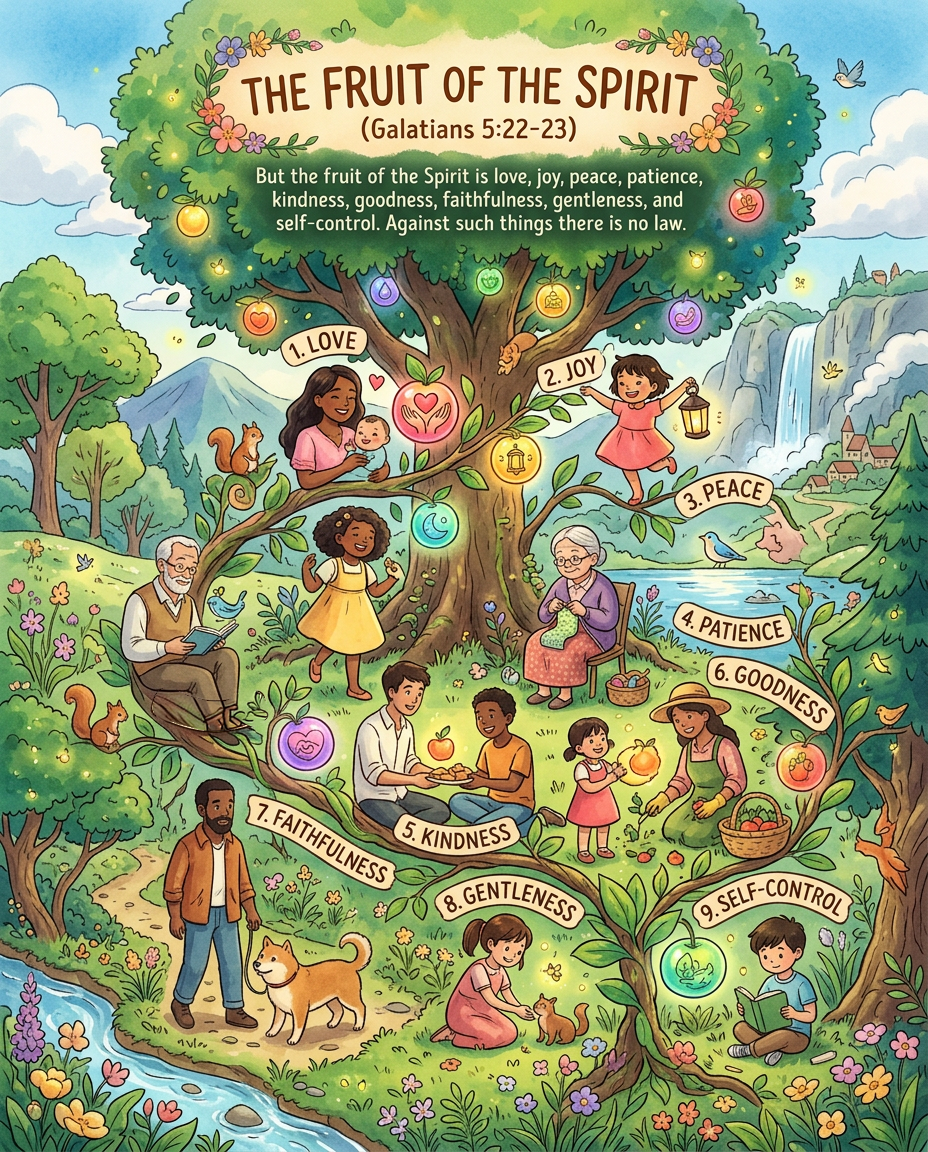
\includepdf[pages=1, fitpaper=false, width=\paperwidth, height=\paperheight, , keepaspectratio=false]{galatians-fruit.png}
\myverse{}Tell me, you that desire to be under the law, don’t you listen
to the law?
\myverse{}For it is written that Abraham had two sons, one by the servant, and one by
the free woman.
\myverse{}However, the son by the servant was born according to the flesh, but the son
by the free woman was born through promise.
\myverse{}These things contain an allegory, for these are two covenants. One is from
Mount Sinai, bearing children to bondage, which is Hagar.
\myverse{}For this Hagar is Mount Sinai in Arabia, and answers to the Jerusalem that
exists now, for she is in bondage with her children.
\myverse{}But the Jerusalem that is above is free, which is the mother of us all.
\myverse{}For it is written,

“Rejoice, you barren who don’t bear.

Break out and shout, you who don’t travail.

For the desolate women have more children than her who has a husband.”\footnote{4:27 Isaiah 54:1}

\myverse{}Now we, brothers, as Isaac was, are children of promise.
\myverse{}But as then, he who was born according to the flesh persecuted him who was
born according to the Spirit, so also it is now.
\myverse{}However, what does the Scripture say? “Throw out the servant and her son,
for the son of the servant will not inherit with the son of the free woman.”\footnote{4:30 Genesis 21:10}
\myverse{}So then, brothers, we are not children of a servant, but of the free woman.


% GALATIANS 5
\mychapter{} \myverse*{}Stand firm therefore in the liberty by which Messiah has made us
free, and don’t be entangled again with a yoke of bondage.

\myverse{}Behold, I, Paul, tell you that if you receive circumcision, Messiah
will profit you nothing.
\myverse{}Yes, I testify again to every man who receives circumcision that he is a debtor
to do the whole law.
\myverse{}You are alienated from Messiah, you who desire to be justified by the law. You
have fallen away from grace.
\myverse{}For we through the Spirit, by faith wait for the hope of righteousness.
\myverse{}For in Messiah Yeshua neither circumcision nor uncircumcision amounts to anything,
but faith working through love.

\myverse{}You were running well! Who interfered with you that you should
not obey the truth?
\myverse{}This persuasion is not from him who calls you.
\myverse{}A little yeast grows through the whole lump.
\myverse{}I have confidence toward you in the Lord that you will think no other way.
But he who troubles you will bear his judgment, whoever he is.

\myverse{}But I, brothers, if I still proclaim circumcision, why am I still
persecuted? Then the stumbling block of the cross has been removed.
\myverse{}I wish that those who disturb you would cut themselves off.

\myverse{}For you, brothers, were called for freedom. Only don’t use your
freedom as an opportunity for the flesh, but through love be servants to one another.
\myverse{}For the whole law is fulfilled in one word, in this: “You shall love your
neighbor as yourself.”\footnote{5:14 Leviticus 19:18}
\myverse{}But if you bite and devour one another, be careful that you don’t consume
one another.

\myverse{}But I say, walk by the Spirit, and you won’t fulfill the lust
of the flesh.
\myverse{}For the flesh lusts against the Spirit, and the Spirit against the flesh;
and these are contrary to one another, that you may not do the things that you desire.
\myverse{}But if you are led by the Spirit, you are not under the law.
\myverse{}Now the deeds of the flesh are obvious, which are: adultery, sexual immorality,
uncleanness, lustfulness,
\myverse{}idolatry, sorcery, hatred, strife, jealousies, outbursts of anger, rivalries,
divisions, heresies,
\myverse{}envy, murders, drunkenness, orgies, and things like these; of which I forewarn
you, even as I also forewarned you, that those who practice such things will not inherit God’s Kingdom.

\myverse{}But the fruit of the Spirit is love, joy, peace, patience, kindness,
goodness, faith,\footnote{5:22 or, faithfulness}
\myverse{}gentleness, and self-control. Against such things there is no law.
\myverse{}Those who belong to Messiah have crucified the flesh with its passions and
lusts.

\myverse{}If we live by the Spirit, let’s also walk by the Spirit.
\myverse{}Let’s not become conceited, provoking one another, and envying one another.


% GALATIANS 6
\mychapter{} \myverse*{}Brothers, even if a man is caught in some fault, you who are spiritual
must restore such a one in a spirit of gentleness, looking to yourself so that you also aren’t tempted.
\myverse{}Bear one another’s burdens, and so fulfill the Torah of Messiah.
\myverse{}For if a man thinks himself to be something when he is nothing, he deceives
himself.
\myverse{}But let each man examine his own work, and then he will have reason to boast
in himself, and not in someone else.
\myverse{}For each man will bear his own burden.

\myverse{}But let him who is taught in the word share all good things with
him who teaches.

\myverse{}Don’t be deceived. God is not mocked, for whatever a man sows,
that he will also reap.
\myverse{}For he who sows to his own flesh will from the flesh reap corruption. But he
who sows to the Spirit will from the Spirit reap eternal life.
\myverse{}Let’s not be weary in doing good, for we will reap in due season if we don’t
give up.
\myverse{}So then, as we have opportunity, let’s do what is good toward all men, and
especially toward those who are of the household of the faith.

\myverse{}See with what large letters I write to you with my own hand.
\myverse{}As many as desire to make a good impression in the flesh compel you to be
circumcised, just so they may not be persecuted for the cross of Messiah.
\myverse{}For even they who receive circumcision don’t keep the law themselves, but
they desire to have you circumcised, so that they may boast in your flesh.
\myverse{}But far be it from me to boast except in the cross of our Lord Yeshua the Messiah,
through which the world has been crucified to me, and I to the world.
\myverse{}For in Messiah Yeshua neither is circumcision anything, nor uncircumcision,
but a new creation.
\myverse{}As many as walk by this rule, peace and mercy be on them, and on God’s Israel.

\myverse{}From now on, let no one cause me any trouble, for I bear the
marks of the Lord Yeshua branded on my body.

\myverse{}The grace of our Lord Yeshua the Messiah be with your spirit,
brothers. Amen.


